\documentclass[12pt]{article}
\usepackage{graphicx} % Required for inserting images
\usepackage{tcolorbox} % For creating colorful boxes
\usepackage{xcolor} % To customize colors
\usepackage[colorinlistoftodos]{todonotes}
\usepackage{amsmath}
\usepackage[utf8x]{inputenc}
\usepackage{geometry}
\usepackage{float}
\geometry{margin=0.8 in}

% Define horizontal rule
\newcommand{\HRule}{\rule{\linewidth}{0.5 mm}}

\begin{document}
\begin{center}

\begin{figure}[h!]
    \hspace*{0 cm} % Negative space to shift the image left
    \includegraphics{BubtLogoByKaniz.png}
\end{figure}
%----------------------------------------------------------------------------------------
\textsc{\Large Computer Science and Engineering }\\[1.5cm]
\textsc{\Large Lab Report}\\[0.3cm]
\textsc{\large Introduction to Linux Operating System}\\[1cm] 
%----------------------------------------------------------------------------------------
\HRule \\[0.4cm]
{ \huge \bfseries OPERATING SYSTEMS\\[0.2cm]  (CSE-210)}\\[0.2cm] % Title of your document
\HRule \\[2cm]

%----------------------------------------------------------------------------------------
\begin{minipage}{0.4\textwidth}
\begin{flushleft} \large
\emph{Submitted By:}\\
Kaniz Fatema \\20245103154\\Intake 53 (01) % Your name
\end{flushleft}
\end{minipage}
~
\begin{minipage}{0.4\textwidth}
\begin{flushright} \large
\emph{Submitted To:} \\
Mishal Al Rahman\\Lecturer\\Dept. of CSE % Supervisor's Name
\end{flushright}
\end{minipage}\\[5cm]

%----------------------------------------------------------------------------------------
%	DATE SECTION
%----------------------------------------------------------------------------------------

{\large August 4, 2025}\\[1cm] % Date, change the \today to a set date if you want to be precise
\end{center}

%----------------------------------------------------------------------------------------
%	Table Of Contents
%----------------------------------------------------------------------------------------

\newpage
\tableofcontents
\newpage

\section*{Scenario}
You are the system administrator of a Linux server used by a small development team. Recently, some team members reported some issues and you need to troubleshoot and perform user management tasks.
%------------------------------------
%	Section 1
%------------------------------------
\section{Troubleshooting}

\subsubsection{Identify the currently logged-in users on the system}
Use the \textbf{who} command to identify the currently logged-in users on the system.
\\ \\ \textbf{\textit {who}}

\begin{figure}[h]
    \centering
    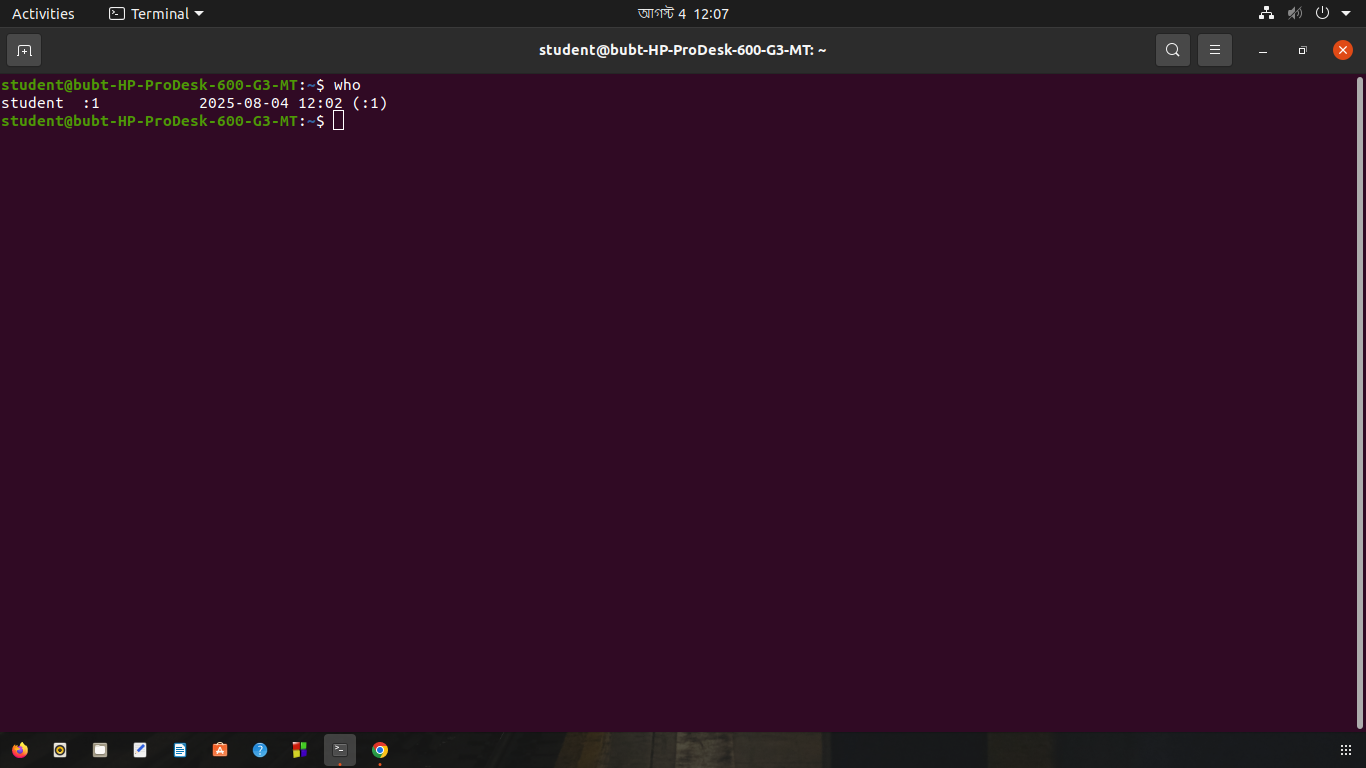
\includegraphics[width=1\textwidth]{1.1.png}
    \caption{Use of the who command}
    \label{fig:kaniz1}
\end{figure}
%------------------------------------
%	Section 2
%------------------------------------
\section{User Management}

\subsubsection{Create a new user named developer1}
Create a new user named \textbf{developer1} using the \textbf{useradd} command.
\\ \\ \textbf{\textit {sudo useradd -m developer2}}

\begin{figure}[h]
    \centering
    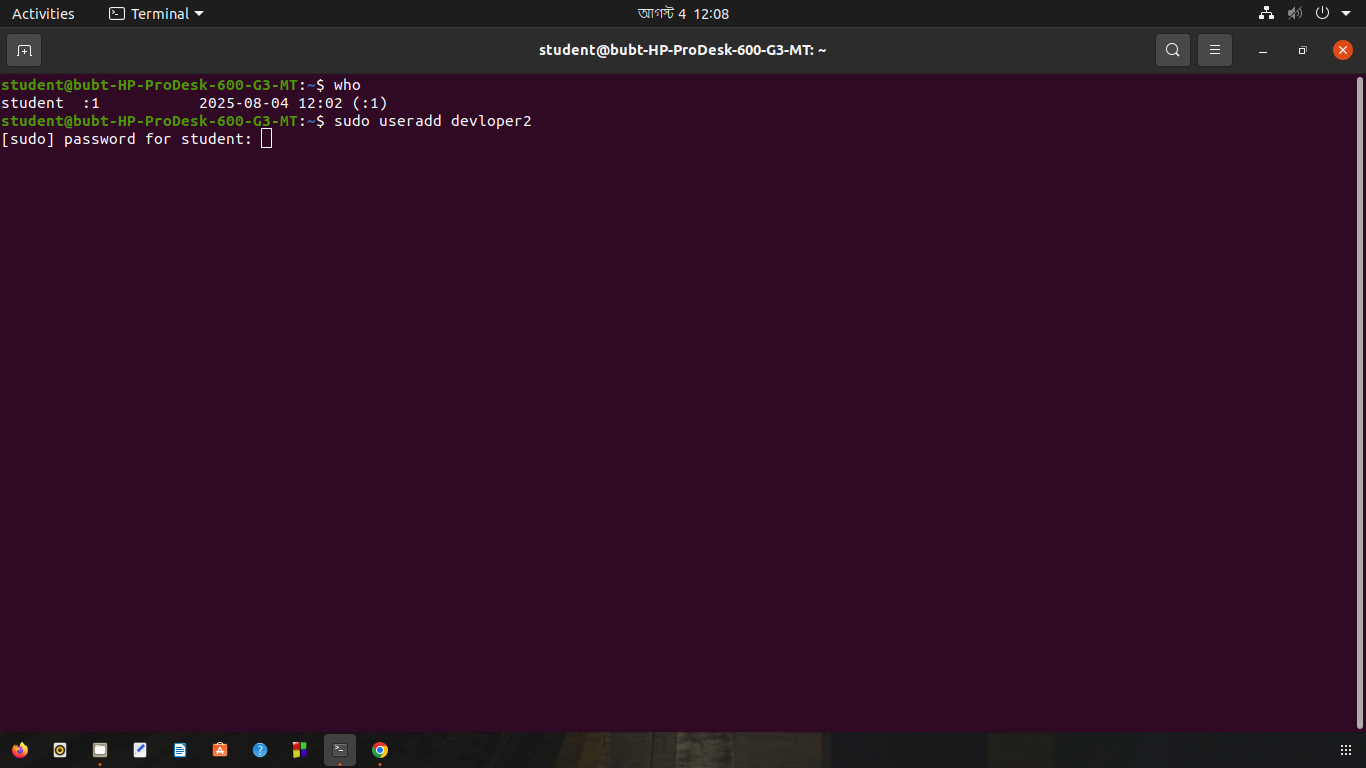
\includegraphics[width=1\textwidth]{2.1.png}
    \caption{Create a new user}
    \label{fig:kaniz2}
\end{figure}

\subsubsection{Set a password for the newly created user}
Set a password for the newly created user using the \textbf{passwd} command.
\\ \\ \textbf{\textit {sudo passwd}}
\\ \textbf{\textit {Example password: 1234}}

\begin{figure}[H] % requires \usepackage{float}
    \centering
    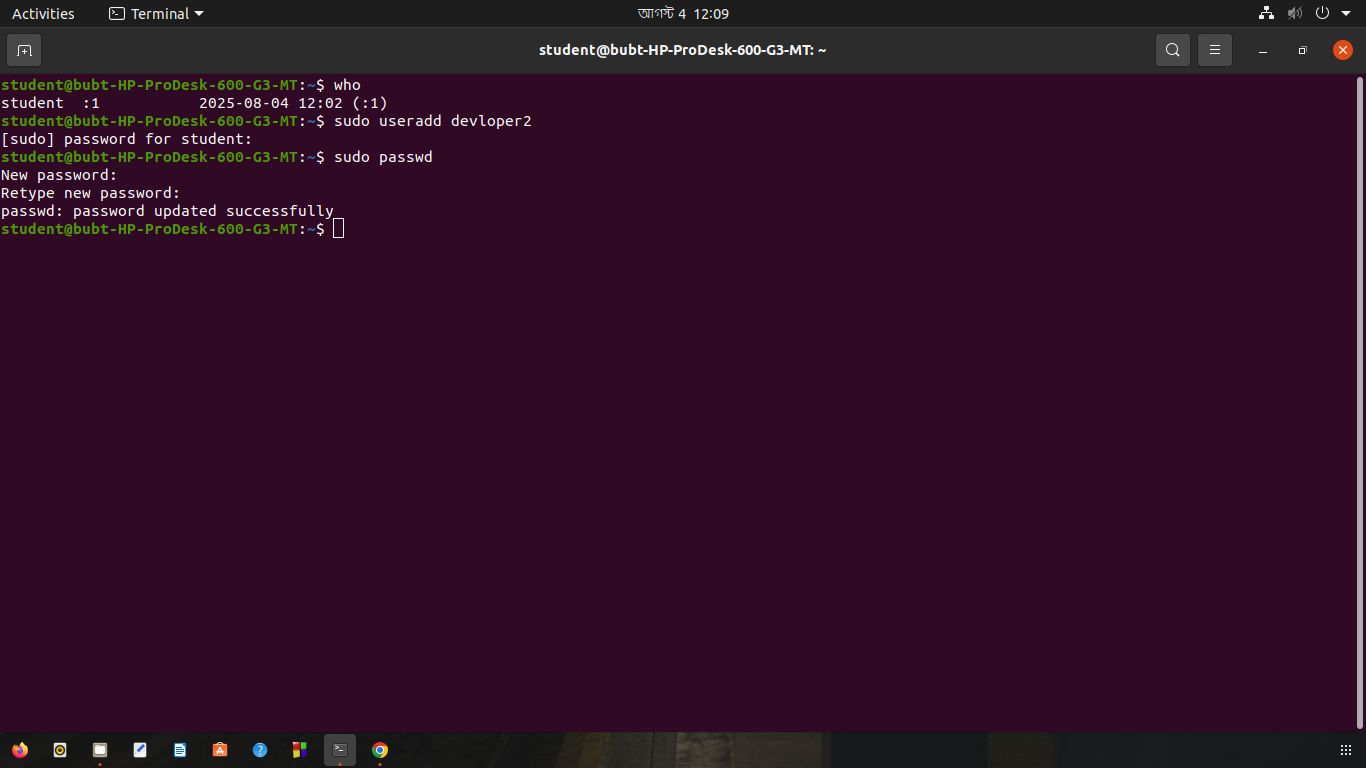
\includegraphics[width=1\textwidth]{2.2.png}
    \caption{Set new password}
    \label{fig:kaniz3}
\end{figure}

\subsubsection{Create a new group named development}
Create a new group named development using the \textbf{groupadd} command.
\\ \\ \textbf{\textit {sudo groupadd development2}}

\begin{figure}[H] % requires \usepackage{float}
    \centering
    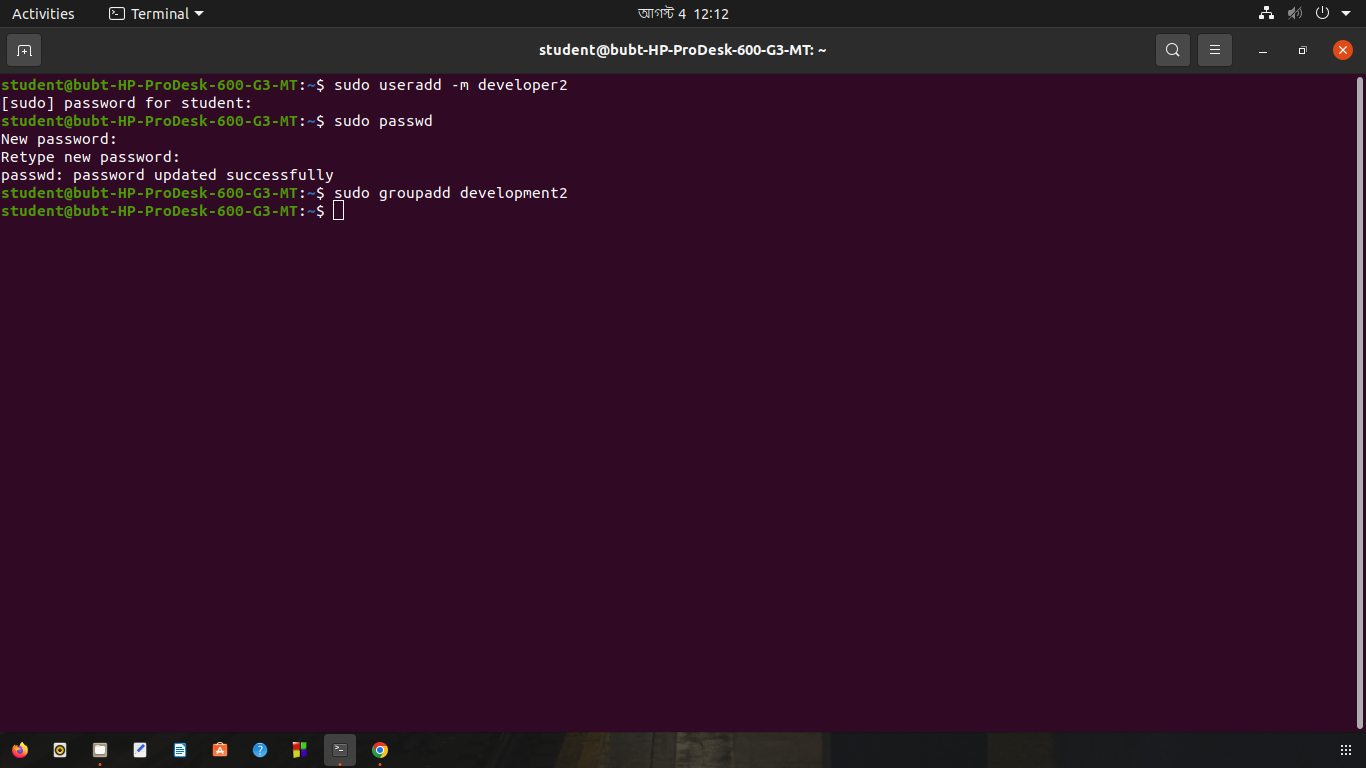
\includegraphics[width=1\textwidth]{2.3.png}
    \caption{Creating a new group}
    \label{fig:kaniz4}
\end{figure}

\subsubsection{Add the user developer2 to the development group}
Add the user developer1 to the development group using the \textbf{usermod} command.
\\ \\ \textbf{\textit {sudo usermod -aG development developer2}}

\begin{figure}[H] % requires \usepackage{float}
    \centering
    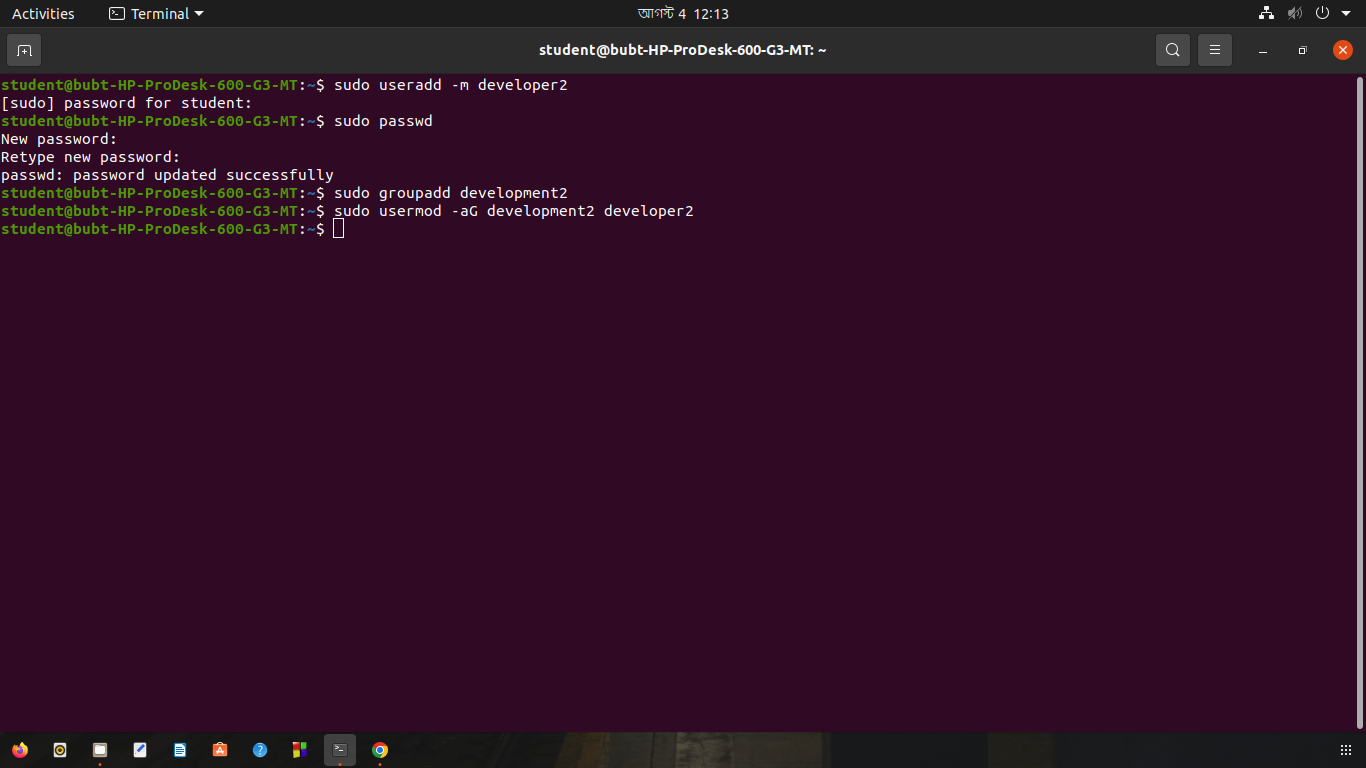
\includegraphics[width=1\textwidth]{2.4.png}
    \caption{Add the user developer2 to the development group}
    \label{fig:kaniz5}
\end{figure}


\subsubsection{Check and display the group memberships of the user developer1}
Check and display the group memberships of the user developer1 using the
\textbf{groups} command.
\\ \\ \textbf{\textit {groups devloper2}}
\begin{figure}[H] % requires \usepackage{float}
    \centering
    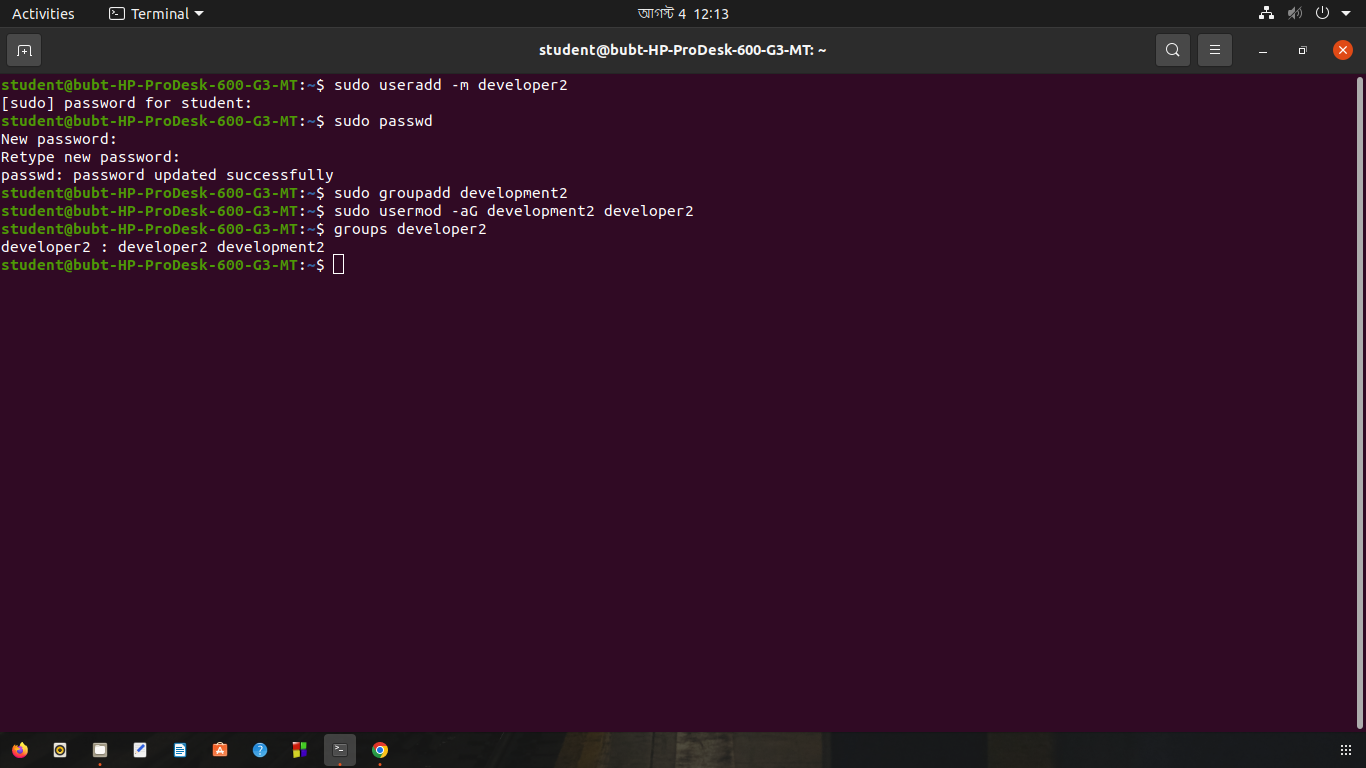
\includegraphics[width=1\textwidth]{2.5.png}
    \caption{display the group memberships}
    \label{fig:kaniz6}
\end{figure}

\subsubsection{Deletion of created user}
Delete the created user from the system
\\ \\ \textbf{\textit {sudo groupdel development2}}
\\ \textbf{\textit {sudo userdel -r developer2}}
\begin{figure}[H] % requires \usepackage{float}
    \centering
    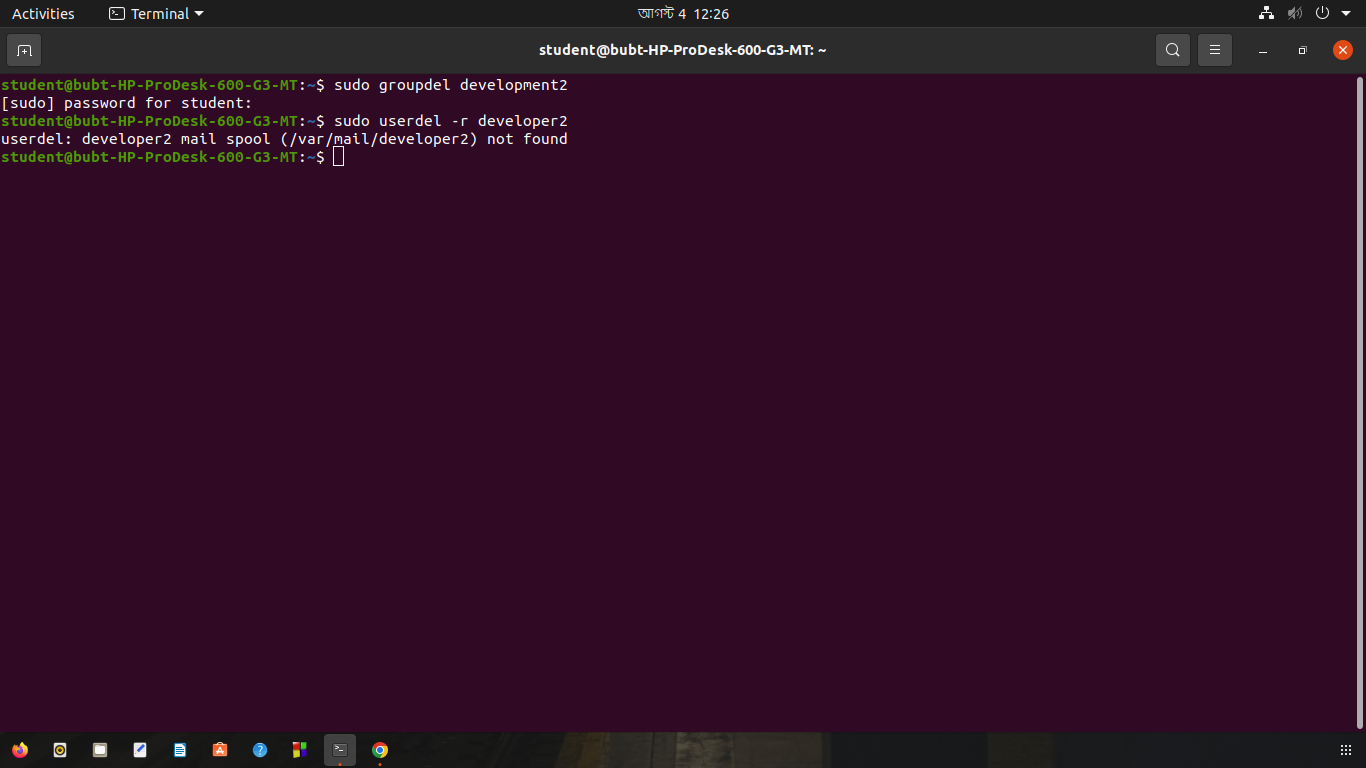
\includegraphics[width=1\textwidth]{2.6.png}
    \caption{Deletion of created user}
    \label{fig:labelname}
\end{figure}

%------------------------------------
%	Section 3
%------------------------------------
\section{File Permission Adjustment}

\subsubsection{Create a directory}
Create a directory named \texttt{project\_files} in the home directory of \texttt{developer1} using the \texttt{mkdir} command.
\\ \\ \textbf{\textit {sudo su - developer2}}
\begin{figure}[H] % requires \usepackage{float}
    \centering
    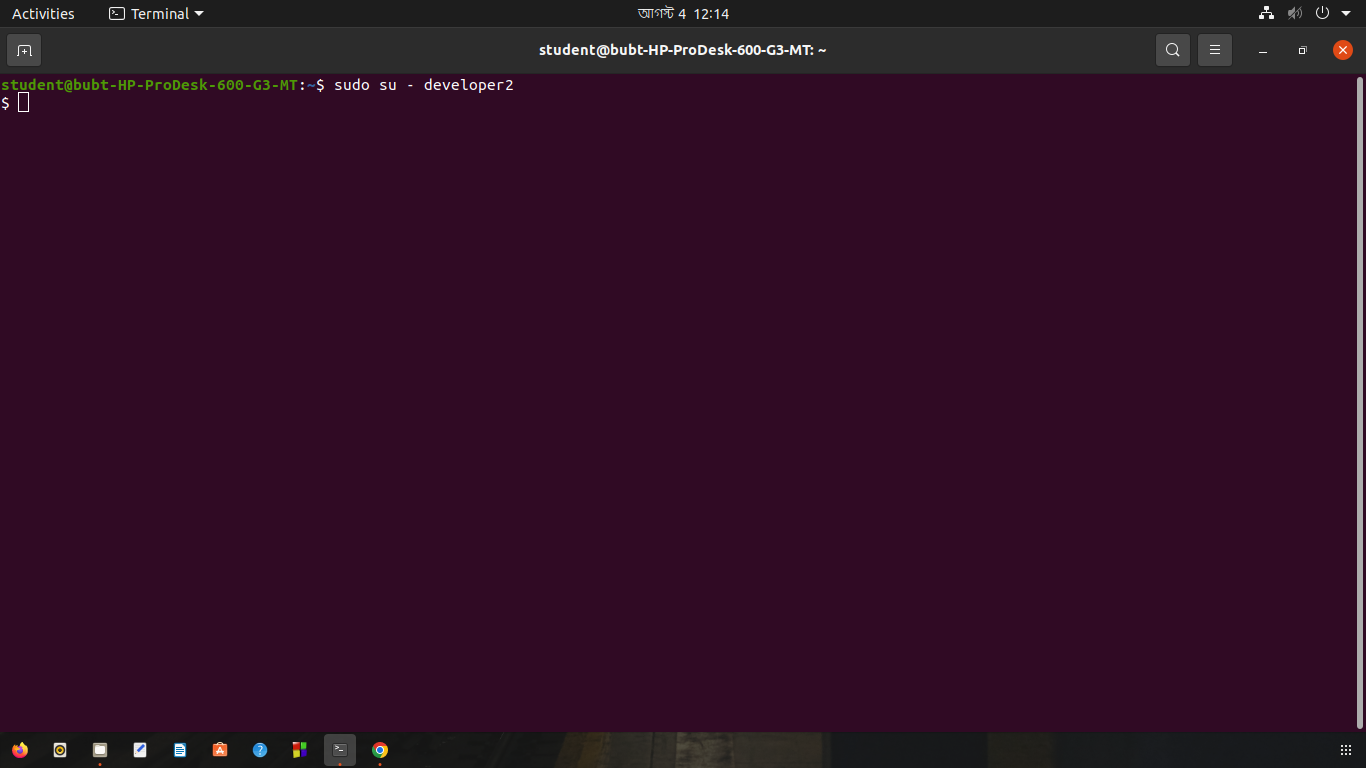
\includegraphics[width=1\textwidth]{3.1.0.png}
    \caption{Logging into the developer2 account}
    \label{fig:labelname}
\end{figure}

\textbf{\textit {who}}
\\ \textbf{\textit {whoami}}
\begin{figure}[H] % requires \usepackage{float}
    \centering
    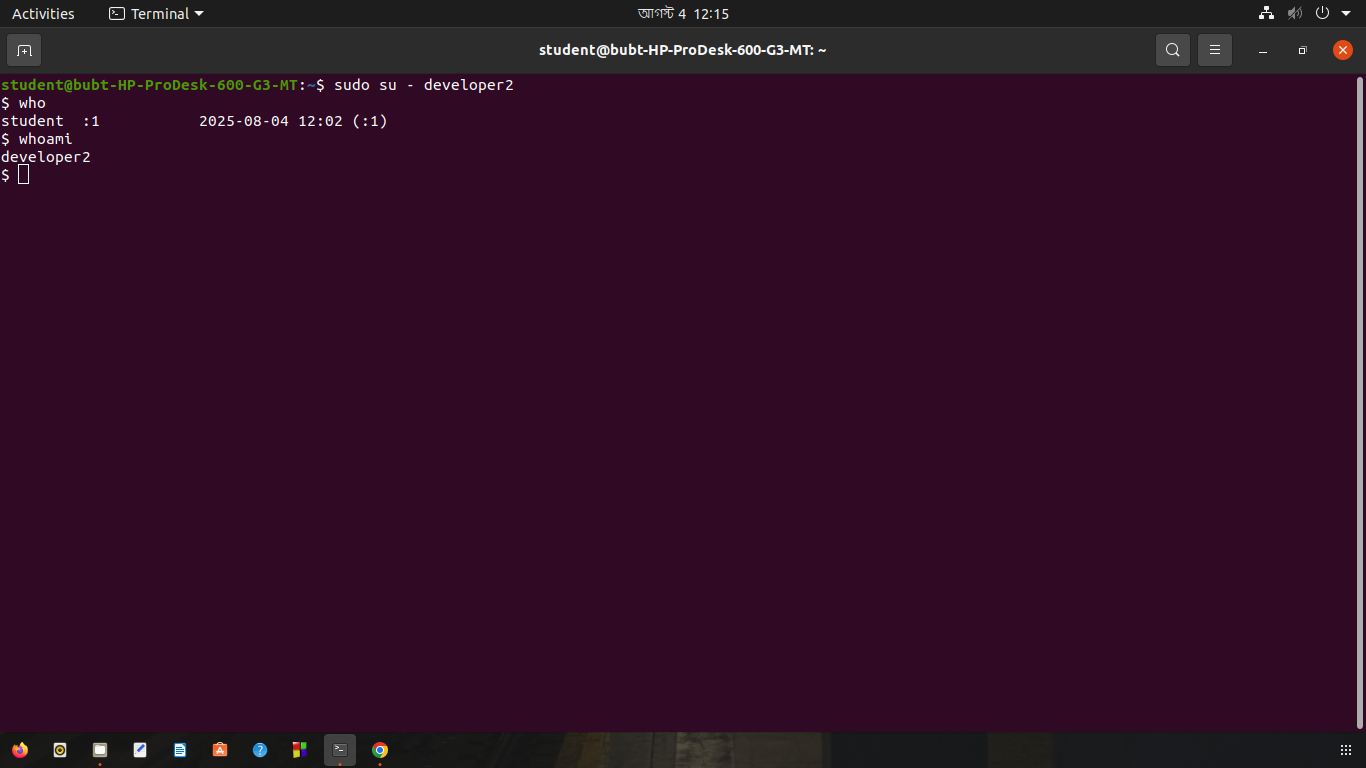
\includegraphics[width=1\textwidth]{3.1.1.png}
    \caption{Verifying that we are in the correct working directory}
    \label{fig:labelname}
\end{figure}

\textbf{\textit {pwd}}
\begin{figure}[H] % requires \usepackage{float}
    \centering
    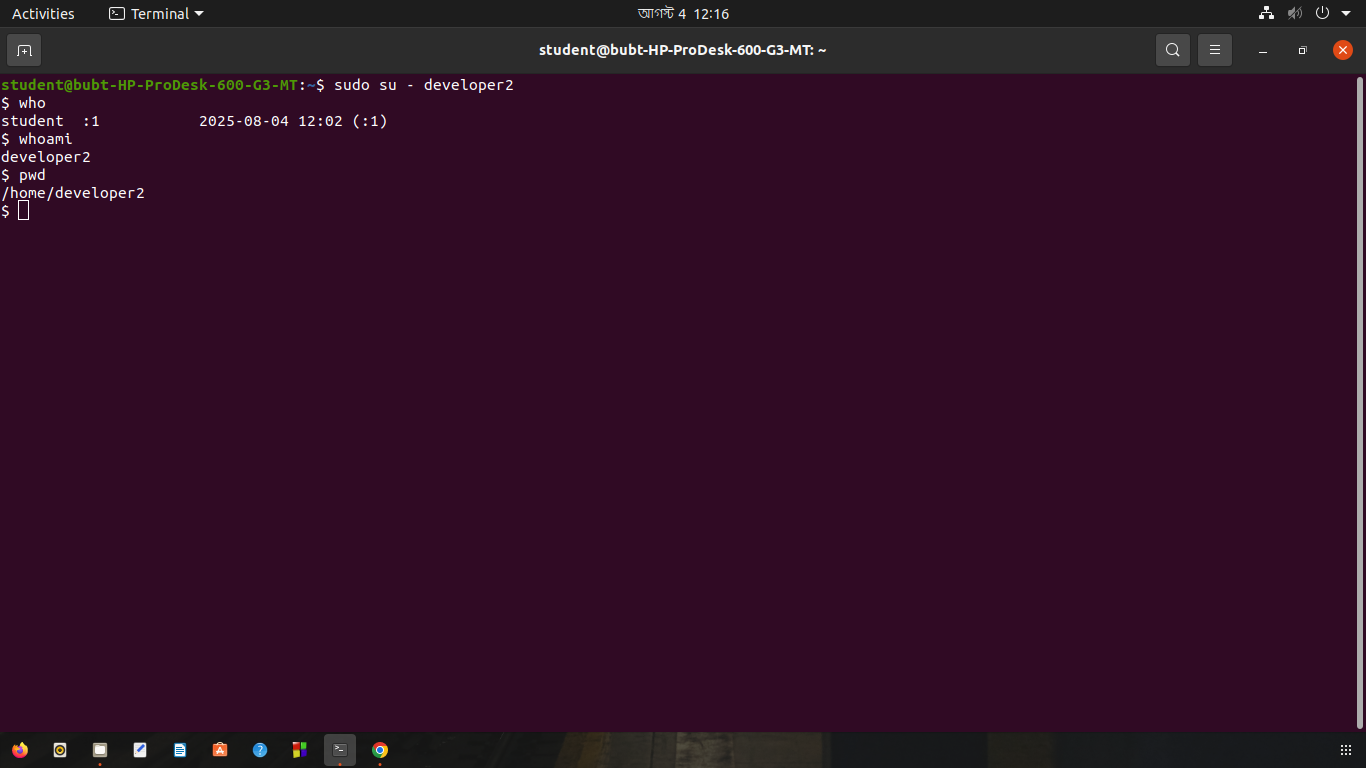
\includegraphics[width=1\textwidth]{3.1.2.png}
    \caption{Verifying if we are logged in as developer2}
    \label{fig:labelname}
\end{figure}

\textbf{\texttt{mkdir project\_files}}
\begin{figure}[H] % requires \usepackage{float}
    \centering
    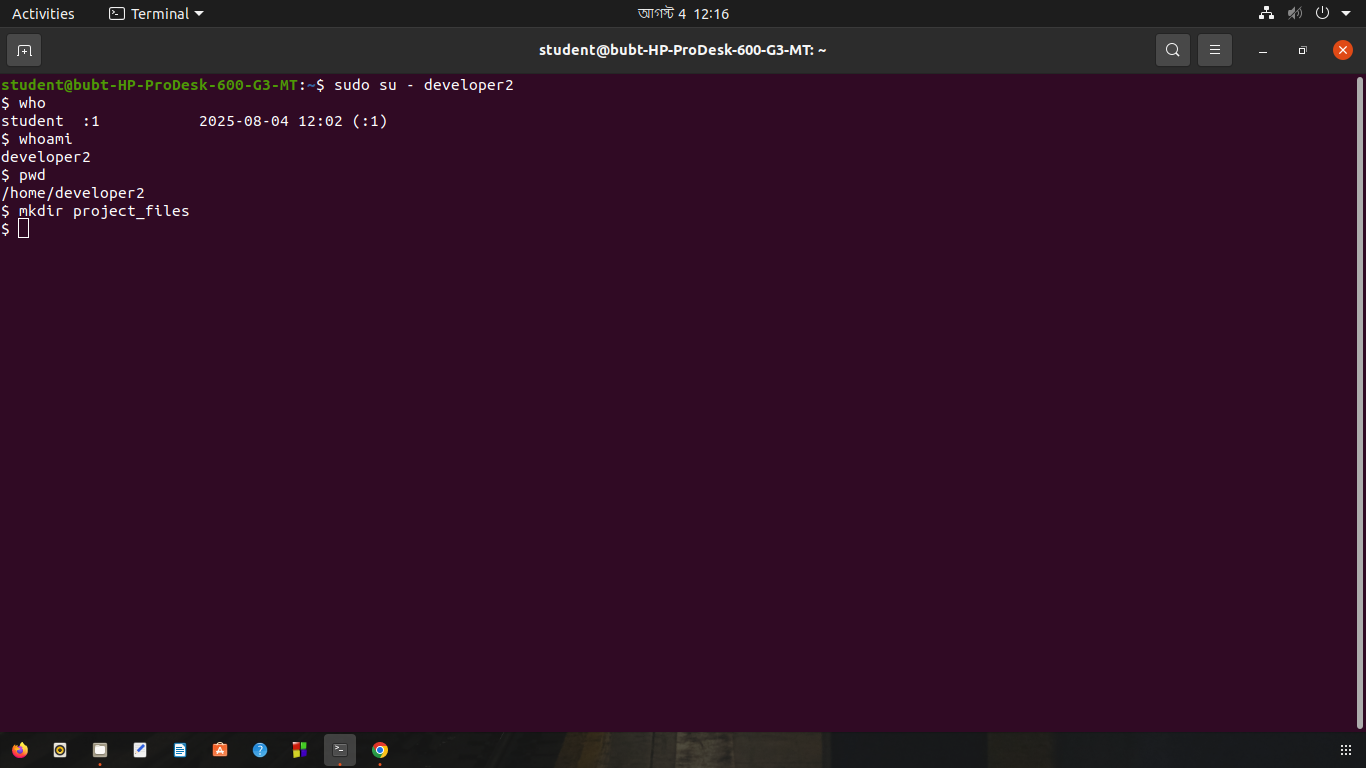
\includegraphics[width=1\textwidth]{3.1.3.png}
    \caption{Creating the projectfiles directory}
    \label{fig:labelname}
\end{figure}


\subsubsection{Change the Ownership}
Change the ownership of the projectfiles directory to developer2 and the group to development2 using the chown and chgrp commands.
\textbf{\texttt{chown developer2 project\_files}} \\
\textbf{\texttt{chgrp development2 project\_files}}

\begin{figure}[H] % requires \usepackage{float}
    \centering
    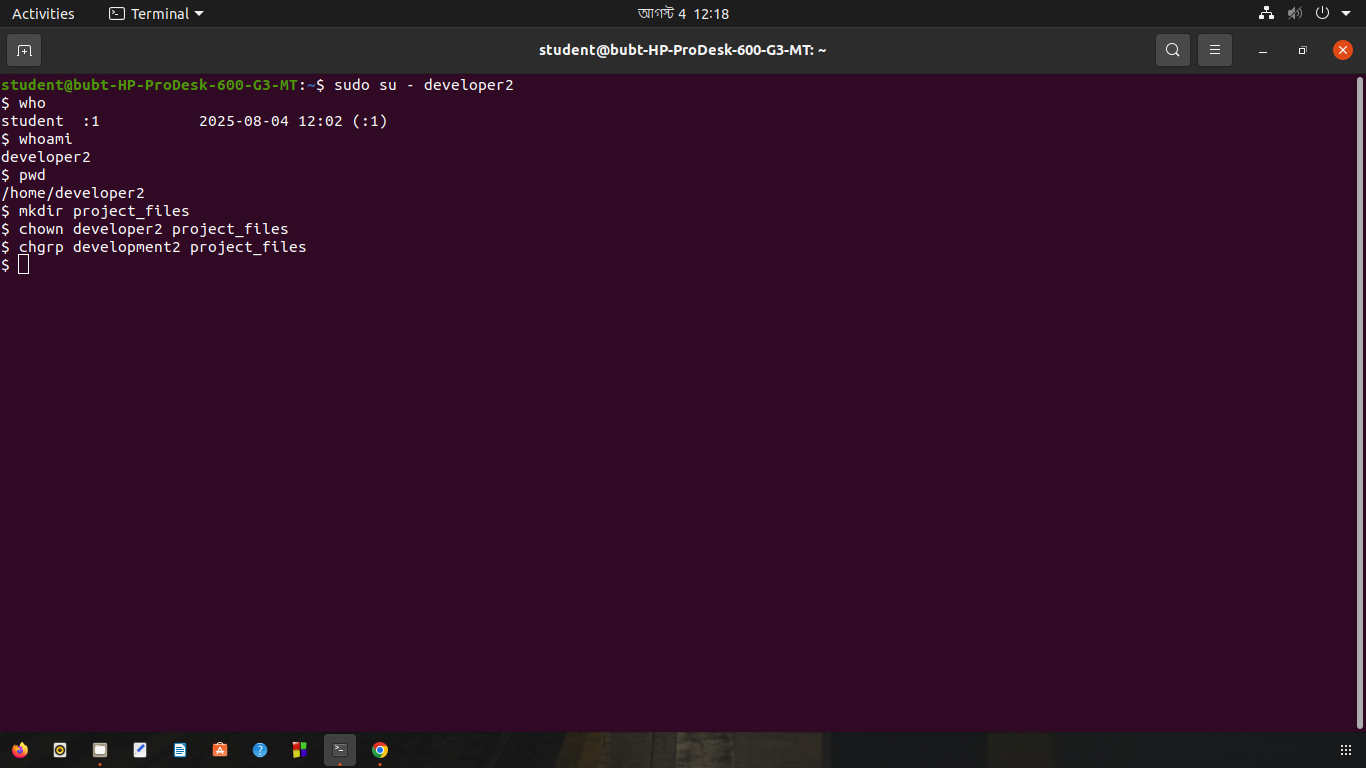
\includegraphics[width=\textwidth]{3.2.png}
    \caption{Change the Ownership}
    \label{fig:projectfiles-directory}
\end{figure}

\subsubsection{Ensure Write Permissions Only to the Owner}

Ensure that only the owner (\texttt{developer2}) has write permissions in the \texttt{project\_files} directory.
\begin{verbatim}
chmod u+w,go-w project\_files
\end{verbatim}

\begin{figure}[H] % requires \usepackage{float}
    \centering
    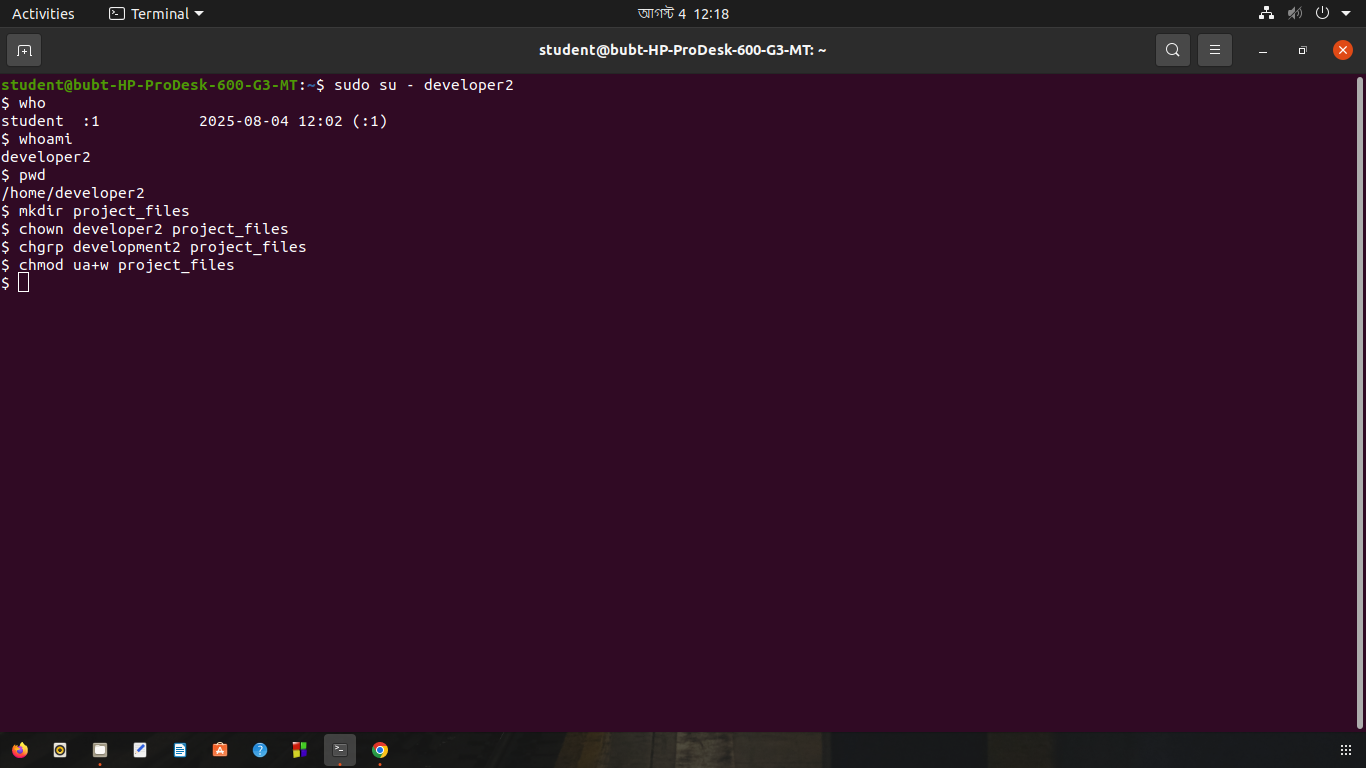
\includegraphics[width=\textwidth]{3.3.png}
    \caption{Ensure write permissions for the owner only}
    \label{fig:write-permissions-owner}
\end{figure}


%------------------------------------
%	Section 4
%------------------------------------
\section{Conclusion}

\subsubsection{Summarize your troubleshooting findings and resolve}
During the setup process, commands such as \texttt{useradd}, \texttt{groupadd}, and \texttt{usermod} required administrative access. 
To execute these commands, we used \texttt{sudo} along with the user's password to gain the necessary privileges.

\begin{verbatim}
sudo userdel developer2
sudo groupdel development2
\end{verbatim}

\subsubsection{Confirm that the new user \texttt{developer2} has been created}
Confirm that the new user \texttt{developer2} has been successfully created, added to the \texttt{development2} group, and that file permissions are set correctly.

\begin{figure}[H] % requires \usepackage{float}
    \centering
    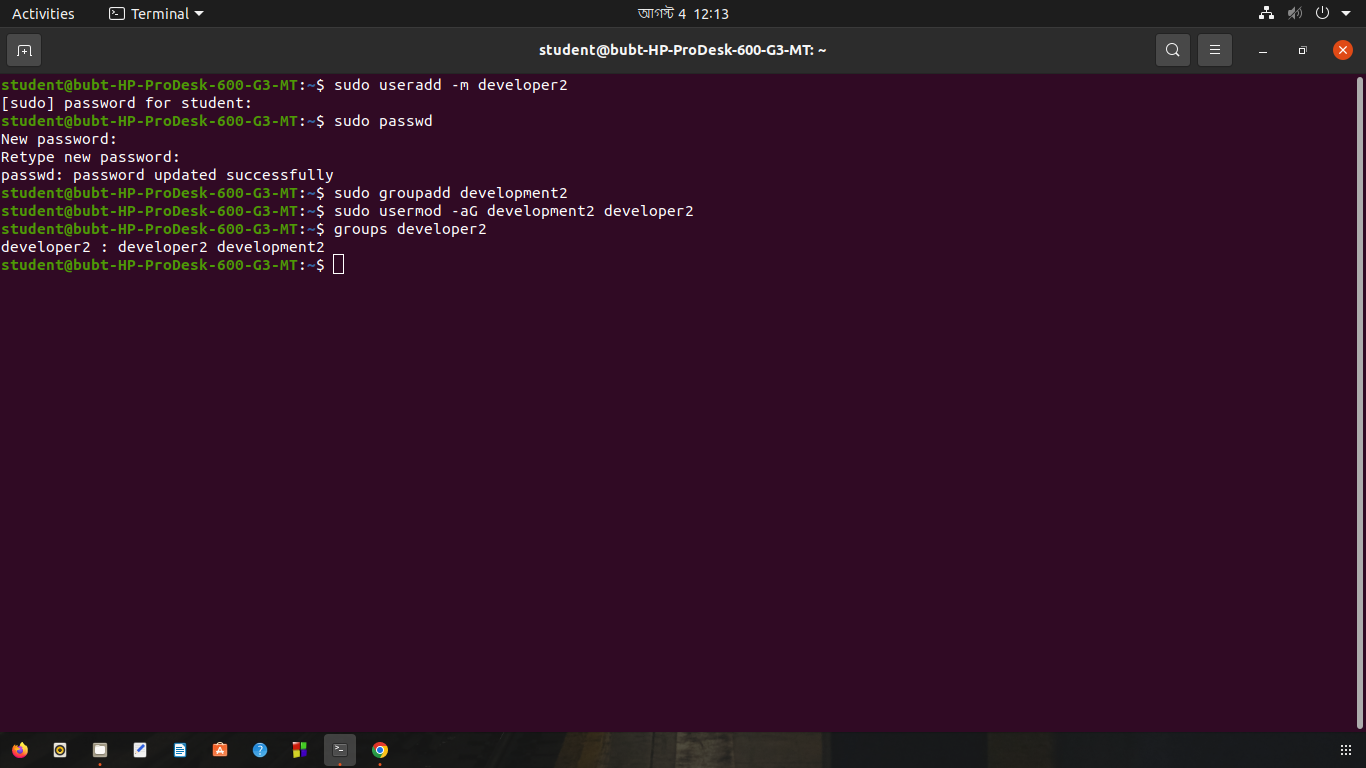
\includegraphics[width=\textwidth]{2.5.png}
    \caption{Verification of the new user \texttt{developer2} and group membership}
    \label{fig:confirm-developer2}
\end{figure}


%------------------------------------
%	Section 5
%------------------------------------
\section{Additional Task}

\subsubsection{Concatenate file1.txt and file2.txt to make a file3.txt}
Concatenate file1.txt and file2.txt to make a file3.txt with all the contents of file1.txt and file2.txt
\\ \\ \textbf{\textit {touch file1.txt touch file2.txt}}
\\ \textbf{\textit {touch file2.txt}}
\begin{figure}[H] % requires \usepackage{float}
    \centering
    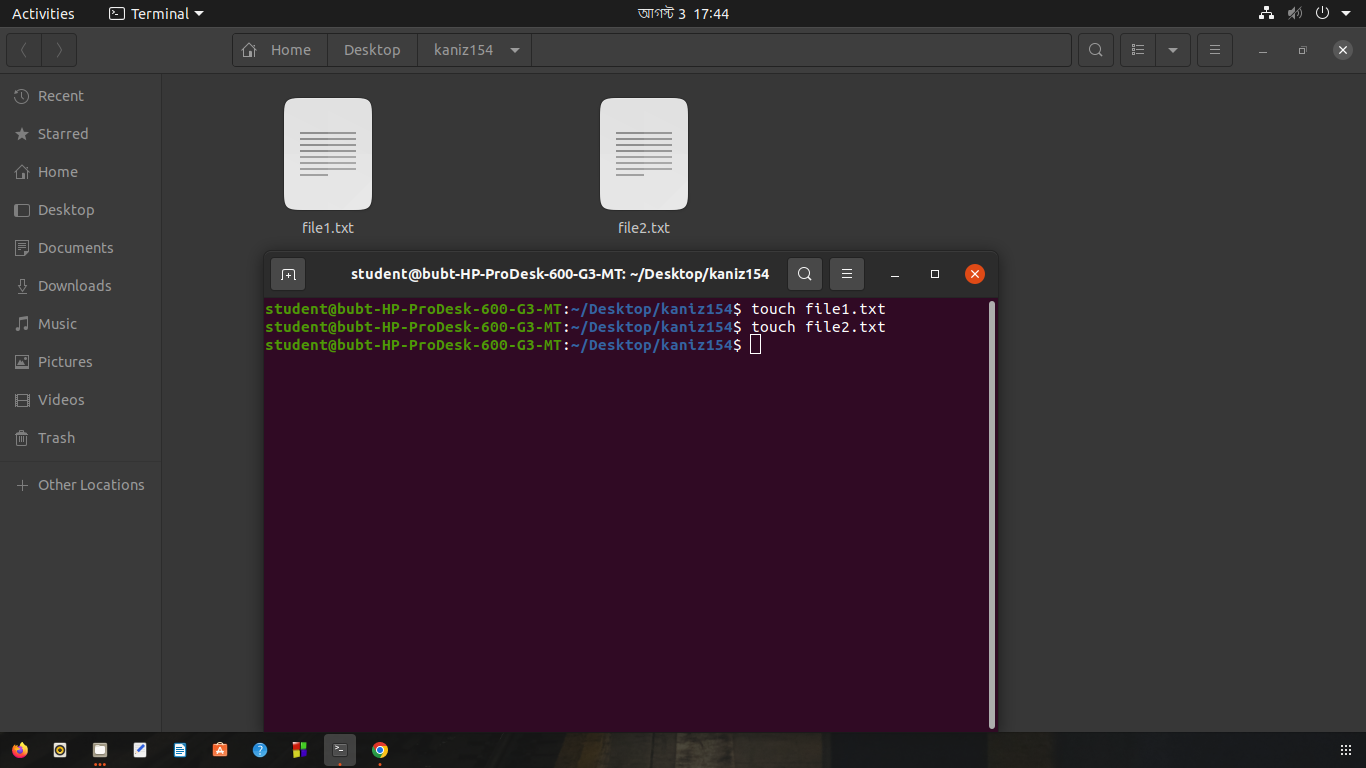
\includegraphics[width=1\textwidth]{5.0.1.1.png}
    \caption{Create file1.txt and file2.txt}
    \label{kaniz 5.0.1.1}
\end{figure}

\textbf{\textit {nano file1.tx}}
\\ \textbf{\textit {cat  file1.txt}}
\begin{figure}[H] % requires \usepackage{float}
    \centering
    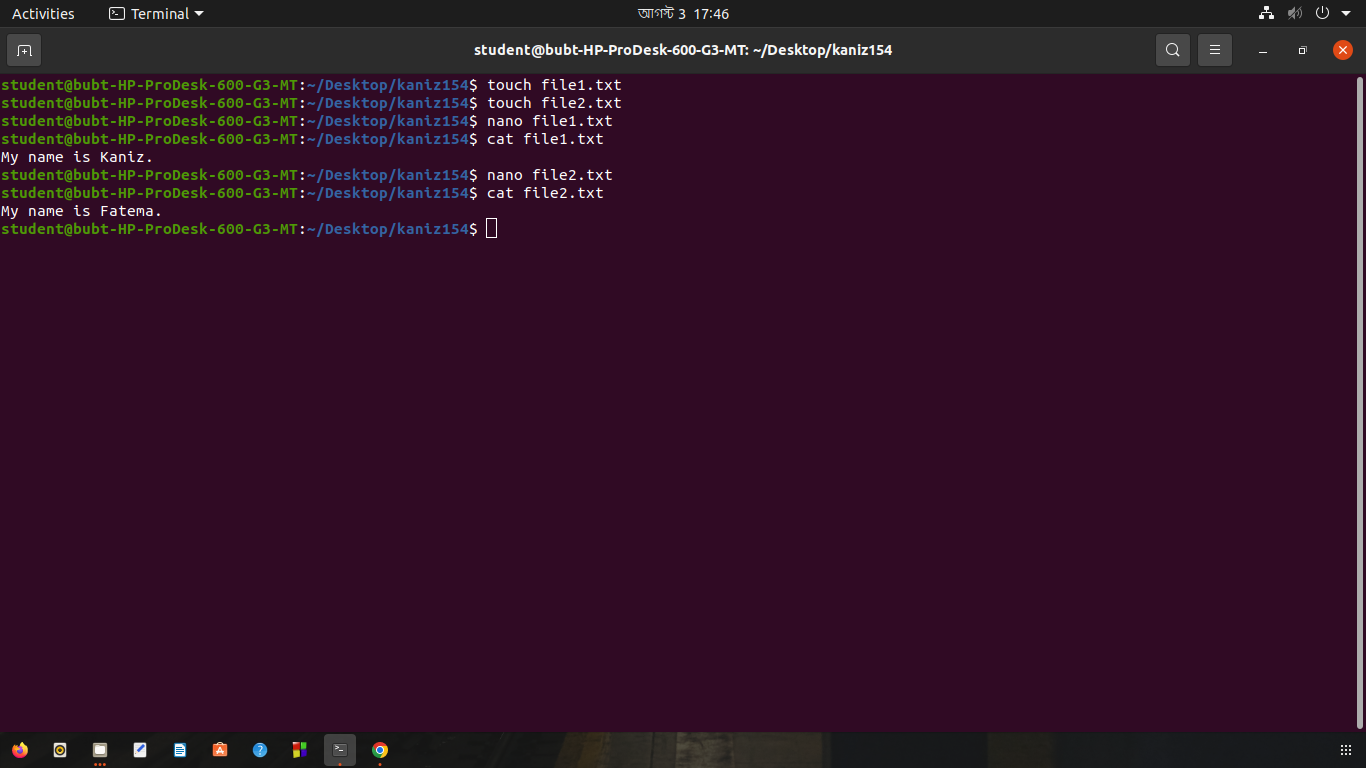
\includegraphics[width=1\textwidth]{5.0.1.2.png}
    \caption{Write and show text file1.txt and file2.txt}
    \label{kaniz 5.0.1.1}
\end{figure}


\noindent
\textbf{\textit{\texttt{cat file1.txt file2.txt > file3.txt}}}\\
\textbf{\textit{\texttt{cat file3.txt}}}
\begin{figure}[H] % requires \usepackage{float}
    \centering
    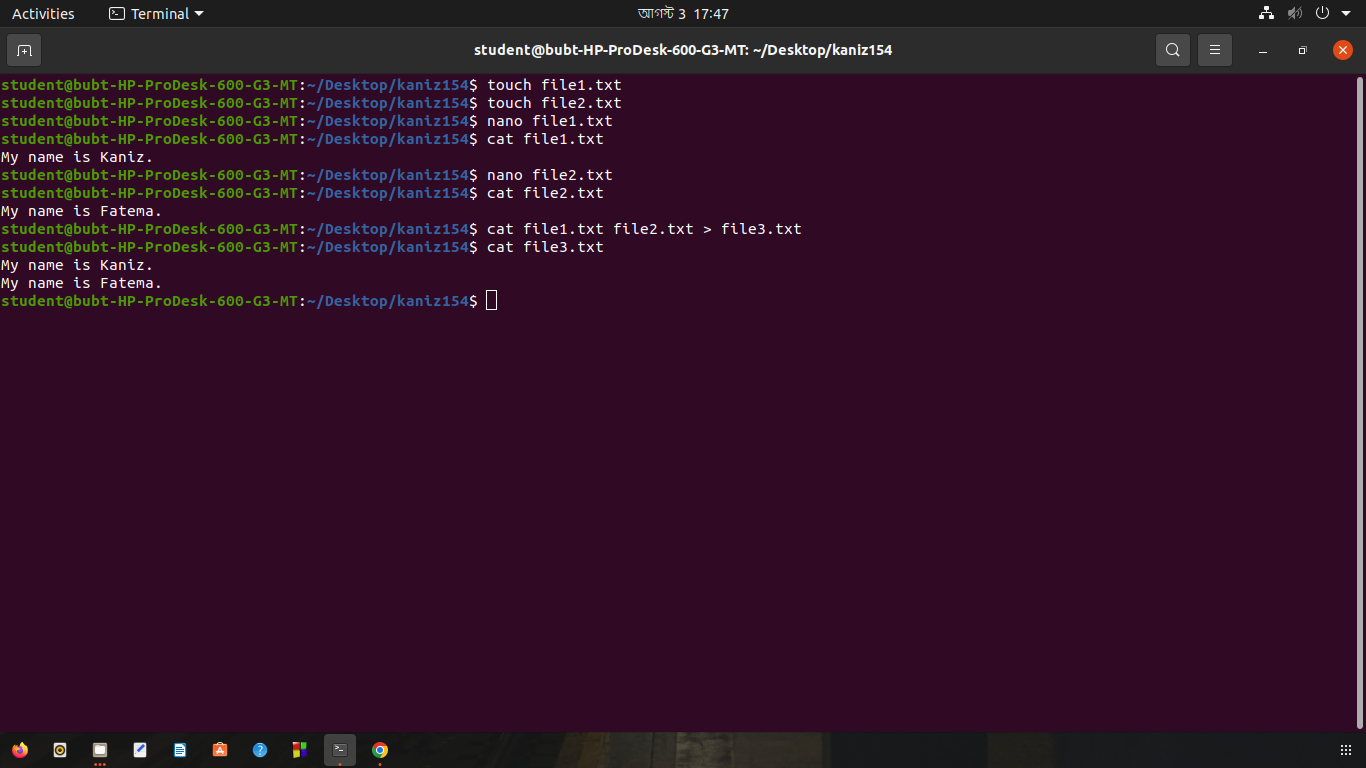
\includegraphics[width=1\textwidth]{5.0.1.3.png}
    \caption{Concatenate file1.txt and file2.txt}
    \label{kaniz 5.0.1.3}
\end{figure}

\subsubsection{Show all your running process list}
To view all running processes on the system, use the command
\textbf{\textit{\texttt{ps aux}}}
\begin{figure}[H] % requires \usepackage{float}
    \centering
    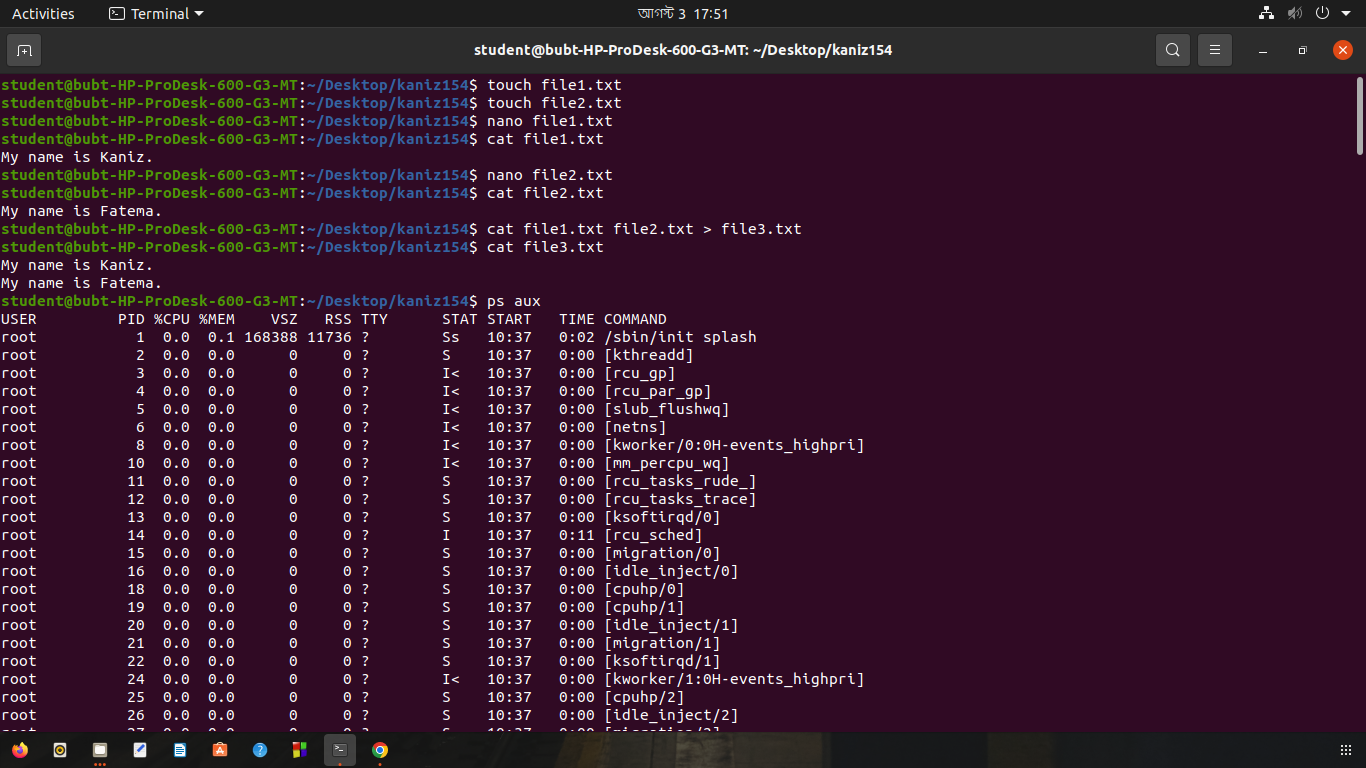
\includegraphics[width=1\textwidth]{5.0.2.png}
    \caption{Show all running process list}
    \label{kaniz 5.0.2}
\end{figure}

\subsubsection{ping google.com}
To check network connectivity, use the command\\
\textbf{\textit{\texttt{ping google.com}}}
\begin{figure}[H] % requires \usepackage{float}
    \centering
    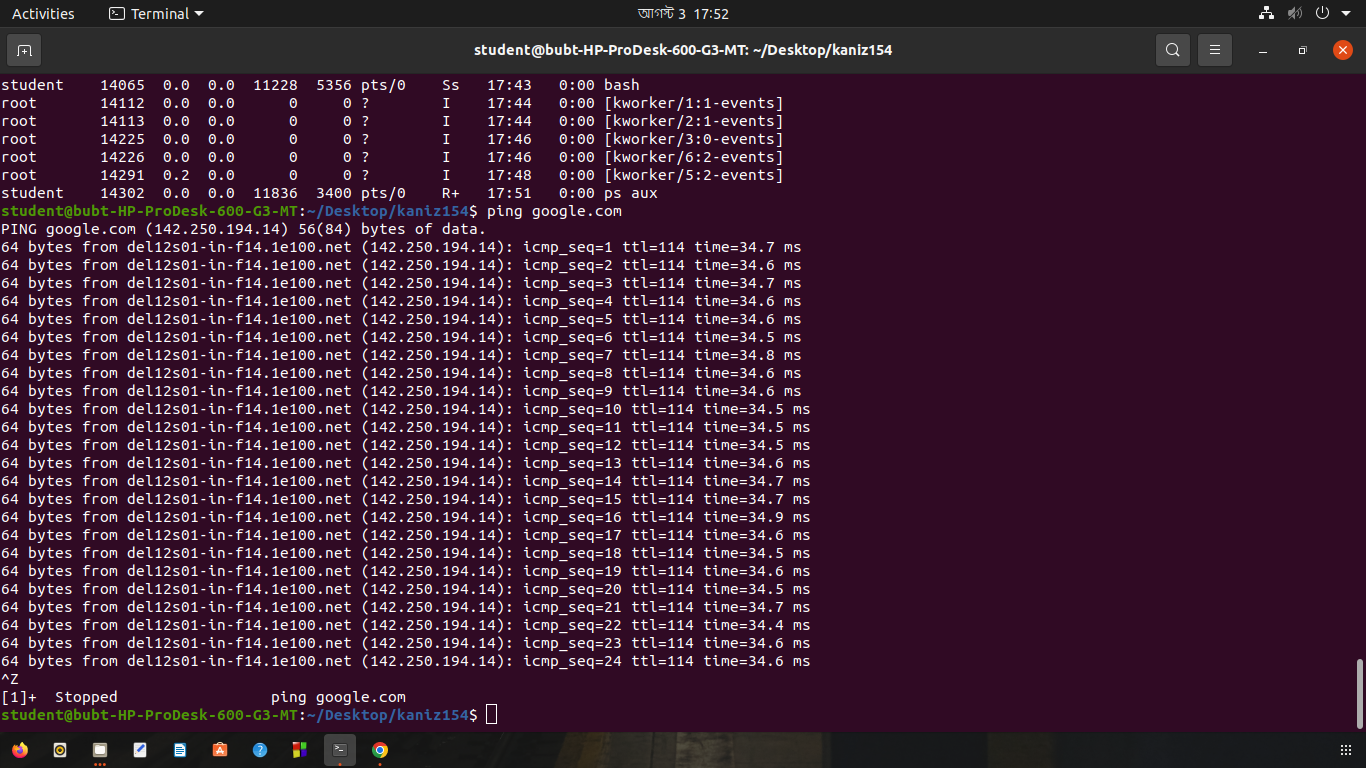
\includegraphics[width=1\textwidth]{5.0.3.png}
    \caption{Show all running process list}
    \label{kaniz 5.0.3}
\end{figure}

\subsubsection{File Zip and Unzip}
To create a compressed archive (tarball) using gzip compression, use the following command
\begin{verbatim}
tar -czvf archive.tar.gz *
\end{verbatim}

\begin{itemize}
  \item \texttt{-c}: create a new archive
  \item \texttt{-z}: filter the archive through gzip
  \item \texttt{-v}: verbose mode, shows progress in the terminal
  \item \texttt{-f}: specifies the filename of the archive
\end{itemize}
To extract the contents of the compressed archive, use:

\begin{verbatim}
tar -xzvf archive.tar.gz
\end{verbatim}

\begin{itemize}
  \item \texttt{-x}: extract files from the archive
  \item Other flags (\texttt{-zvf}) are the same as above
\end{itemize}

\begin{figure}[H] % requires \usepackage{float}
    \centering
    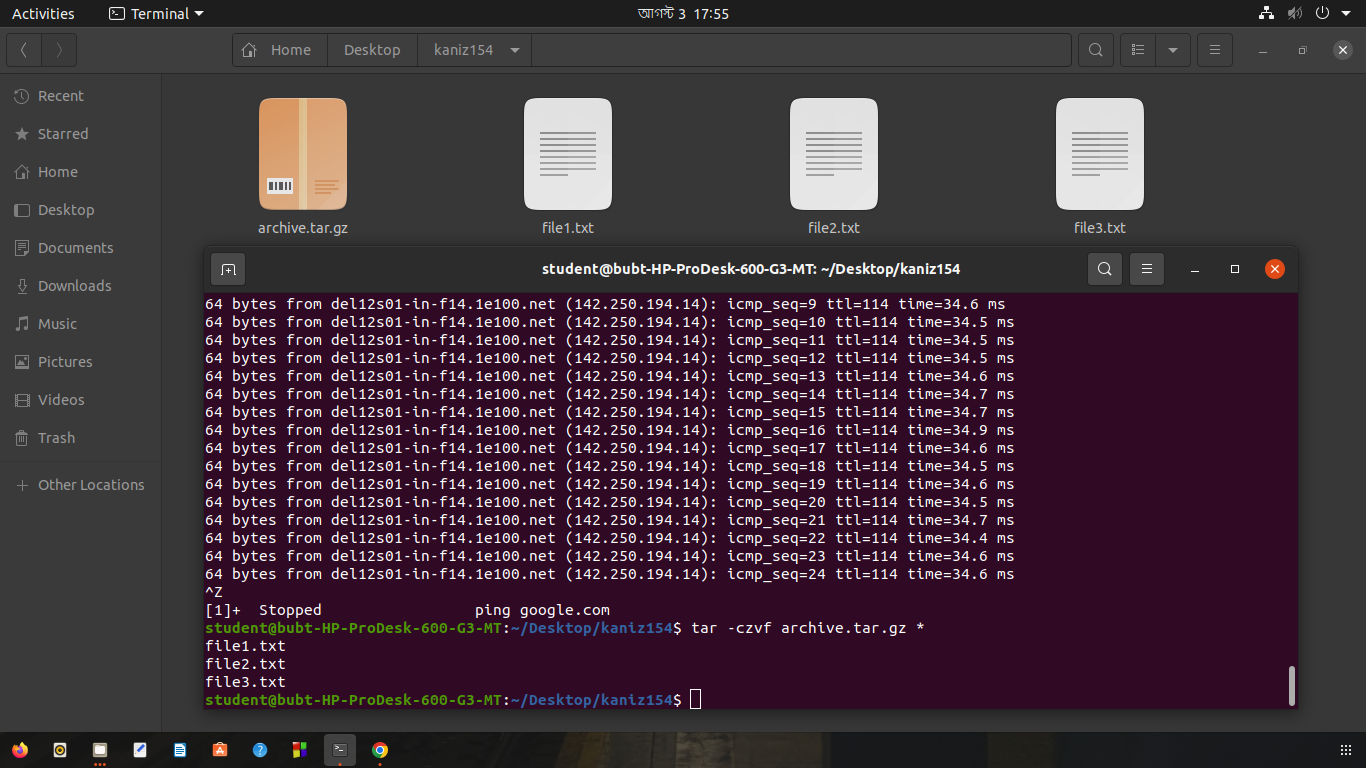
\includegraphics[width=1\textwidth]{5.0.4.png}
    \caption{File Zip and Unzip}
    \label{kaniz 5.0.4}
\end{figure}

\footnote{Kaniz Fatema }
\footnote{ID: 20245103154 }
\end{document}